% #############################################################################
% This is Chapter 2
% !TEX root = ../main.tex
% #############################################################################
% Change the Name of the Chapter i the following line
\fancychapter{Problem Definition}
\cleardoublepage
% The following line allows to ref this chapter
\label{chap:problem}

This chapter will define the problem, the client requirements and list the necessary functionalities of the solution, to successfully address the problem.
First some context surrounding the problem is given. 
Next, the profile of the target clients will be described, and some examples will be given.
The following section contains a list of client requirements the solution must abide by.
Then it will shed the ligh on some essential concepts in order to understand the operations that need to be implemented.
It will end by detailing the client use cases it must provide.

As discussed before, the same computers commonly used for communications and information storage are exploitable by attackers, and can cause a minor inconveniences, to possibly severe repercussions, such as, losing your confidential data to malicious parties.

An interesting approach to improve security is to add another layer of security to confidential data and communications through the addition of an device, independent of the user's personal computer. The device is responsible for the security of sensitive data and communications.

% An illustration of the system with multiple users can be seen in figure~\ref{fig:main-system}.

\subsection{Entities}\label{chap:problem:entities}

These type of devices are especially relevant to people high responsibility jobs, that handle very sensitive information, which have dire consequences if they are lost, corrupted or leaked.
Some examples are government officials who handle confidential information pertaining to a country, company executives, such as the CEO who have access to company secrets, diplomats who manage confidential treaties, and military officers who have access to information critical to a countries' security.

% Talk about groups and individuals
Additionally, not just individuals have interest in these systems, a device can be assigned to a group of people representing an entity. For example, in the armed forces, a device can be assigned to the navy, one to the infantry, and every other faction. Any ranked officer, or people with a certain level of authority, could use the entity device, to communicate with other people or entities, in behalf of the group.

\subsection{Devices}\label{chap:problem:devices}
% Devices
There are currently on the market some dedicated devices designed to secure communications and save private data.
These type of devices have physical tamper-resistant measures against attackers who wish to read the device's information. They also provide fail-safe mechanisms in case of an attack.
\ac{HSM} is a high grade device, with more computational power and larger storage capacity for the user's secrets.

Smart Cards, provide secure and portable tamper-resistant storage.
They have lower processing power, and smaller memory which only allows to store a small amount of data.
They have a low-cost, so can be produced in bulk and easily replaced. Only an RFID card reader is needed to read its information, and verify the owner's identity.
Because of these features, they are widely used in the retail, healthcare, communication and government industries.


% -----------------------------------------------------
% -----------------------------------------------------
\section{Client Requirements}\label{chap:problem:requirements}

To effectively address the presented problem, there are several high-level requirements the solution must adhere to:
\begin{itemize}
	\item Devices should be distributable to either individuals, entities composed of multiple people or groups of people;
	\item The system must allow communications between groups of people and individuals representing themselves or an entity;
	\item The system must be responsible for securing all communications against disclosure, tampering or any sort of attacks;
	\item The device should be dependent from user's personal computers. This way, the user's do not need to worry about what computer they use, the device is responsible for providing all the functionality;
	\item Users should be able to choose who they want to initiate secure communications. The application should provide the functionality to allow this;
	\item Is should be simple to use by everyone, including non-technical people;
	\item It should have a relatively low cost, enough to allow distribution of several devices between multiple individuals and groups;
	\item Only individuals with a certain level of clearance should be authorized to use the device. Personal devices should only be accessible by their owners.
\end{itemize}

% TODO
These client requirements need to be translated into slight more technical and tangible requirements a possible solution must have.

% -----------------------------------------------------
\subsection{Communications}\label{chap:problem:services:comms}
In order to secure communications, the following services must be guaranteed: confidentiality, integrity and authentication.
The system can give an option to provide non-repudiation to documents or files, by means of digital signatures.
% falar de cartao do cidadao

% -----------------------------------------------------
\subsection{Key management}\label{chap:problem:services:key}
The device must store all the symmetric and asymmetric keys related to the entity or individual who owns the device.

The device must support secure storage in order to store the user's sensitive information, such as the cryptographic keys used for communication.
Additionally, the device should have physical tamper-resistant measures and mechanisms in place, in case of an intrusion, such as, permanent erasure of all sensitive data. 
This means that even if an attacker is in possession of the physical device, it should be extremely difficult or even impossible to extract any information from it.

These keys must never be exposed to the outside environment of the device to ensure the security of communications and independence of the system.

All cryptographic operations must also be performed inside the device.

Importation of other user's public keys.

Each entity has one pair of asymmetric keys, stored in their device, a private and a public.

% -----------------------------------------------------
\textbf{\ac{PKCS} \#11} are a group of widely used cryptographic standards, which define an \ac{API} designed to manipulate common cryptographic objects, such as keys.
With this \ac{API}, the objects can be used, created and modified by applications, without exposing them to the application's memory.
The solution should follow this standards, to strengthen its security requirements.

% -----------------------------------------------------
\subsection{Usability}\label{chap:problem:services:usability}
There are also several usability requirements the solution must abide by.

% -----------------------------------------------------
\subsubsection{Device Standardization}

The solution should work with a plethora of devices, which will increase the adoptability of the solution among clients. This entails the use of a widely established protocol, which clearly defines a set of functions and standards the system should follow.
This is where the \ac{PKCS} \#11 standard is again relevant. It allows operations to be standardized across different devices, increasing the range of supported devices. By implementing the system in accordance with these guidelines, it will have a higher device interoperability.

% -----------------------------------------------------
\subsubsection{Client Application}

The system should provide an application on the user's device, which will communicate with the physical device, and make the operation's available to the user through a simple interface for the regular non-tech savvy user.

Another related requirement is the usage of a common connection solution, e.g. USB cable, to further increase the pool of supported devices.

In addition, the system should perform the operations in a reasonable time to minimize the user's wait, and improve the user experience.

% -----------------------------------------------------
% -----------------------------------------------------
\section{Concepts}\label{chap:problem:concepts}

In this section some necessary concepts will be explained in order for non-technical users can easily understand the background, as well as the necessary concepts to fulfill the previously defined requirements.

Some services are crucial, in order to guarantee the security of communications.
\textbf{Confidentiality} is a security service which keeps the contents of communications secret, except from the authorized parties.
\textbf{Integrity} safeguards communications from modifications by attackers.
The \textbf{authentication} service can verify the identity of an agent, taking part in the communications.
Finally the \textbf{non-repudiation} service prevents an entity from denying authorship of a piece of information.

\textbf{Cryptographic keys} are tools used to grant the aforementioned services. Users in possession of the keys can secure and access their messages.
\textbf{Symmetric keys}, in possession of all communicating parties, are used to secure messages and documents.
\textbf{Asymmetric key pairs} (public and private key), are used to enable communicating by for example, sharing new symmetric keys between users who wish to communicate. Secondly, they provide non-repudiation through digital signatures.
These keys identify the owner. The private key must always be in possession of the owner. With it they can prove their identity and generate signatures.
The public key should be shared with other people so that they can share keys and verify the owner's signatures.

\textbf{Digital signatures} are a digital version of handwritten signatures, commonly used anywhere forgery detection is essential, for instance in financial transactions.
Qualified signatures are a special type of signatures where the private keys are generated and stored inside a device, such as a Smart Card, and never leave it.
This strong signature legally represents a person or a group. This type of signatures are used in the Portuguese Citizen Card.

% -----------------------------------------------------
% -----------------------------------------------------
\section{Use Case Scenarios}\label{chap:problem:scenarios}

% -----------------------------------------------------
% -----------------------------------------------------
\section{Context}\label{chap:problem:context}

\begin{figure}[h]
    \centering
    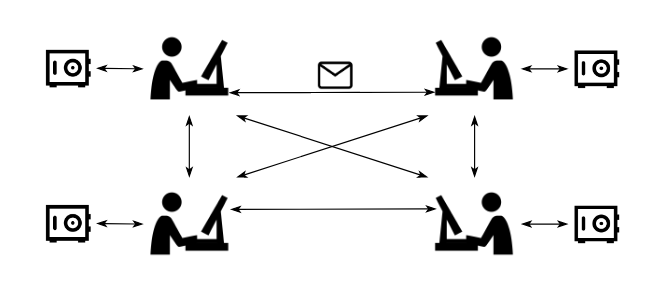
\includegraphics[width=0.7\textwidth]{./Images/main-figure.png}
    \caption{System illustration.}
    \label{fig:main-system}
\end{figure}

This section will define and detail the use cases the solution must satisfy and provide to the user. The combination of the use cases satisfy the client requirements in section \ref{chap:problem:requirements}.
Figure \ref{fig:main-system} will be used as an example and illustration for the different scenarios.

% -----------------------------------------------------
\subsection{Initial State}\label{chap:problem:scenarios:init}

The users will receive the device with a pair of asymmetric keys, a private and public, generated inside the device from fabric.
Each device will have the user's public keys, whom he wishes to communicate.
The user can request whose public keys he wants, before the device is initialized in fabric.
This allows the users to share symmetric keys between them, which they can user to begin trading data securely.
The device can also come with the symmetric keys already shared and stored in each user device.

% -----------------------------------------------------
\subsection{Authentication}\label{chap:problem:scenarios:auth}

Every user must authenticate himself, before using the device. This can be done by providing a \ac{PIN}, which the device will verify before unlocking the session for the user.
The device will come from fabric with a default authentication \ac{PIN}. The users should be allowed to change this number.

For \textbf{personal} devices, there is only one user, the owner, as illustrated by Alice and Bob in figure \ref{fig:main-system}. There is only the single authentication \ac{PIN}, which when sent to the device, unlocks the session, and the user can access its services.
For \textbf{groups} and entities, there can be multiple users, illustrated by Charlie. In this case, there are different scenarios for authentication.
The simplest is when it is not needed to authenticate the individual user, only the entity. There is only a single authentication \ac{PIN} for the entity. All the user's with permission to communicate in behalf of the entity, must know the \ac{PIN}. They only need to send the number to the device to be allowed access to its operations.

The second scenario, is when an entity wishes to authenticate each individual user with access to the device. 
This would entail a more complex process. A user will be assigned the role of administrator. For example, in the military, this could be assigned to the top ranking general. The administrator, using the \ac{PIN} from fabric, is able to register new users with their own private \ac{PIN}, access the logs of which user logged in and when, as well as, which messages they sent and received.
The registration of a new user must be done physically with both administrator and user. The administrator authenticates himself to the device, begins the registration process and allows the user to insert their name and \ac{PIN}.
It is important to note that in all scenarios, only the users or the entity is authenticated, the device does not authenticate itself to the user.

% -----------------------------------------------------
\subsection{Communications}\label{chap:problem:scenarios:comms}

For each channel of communication between individual users, groups or entities, the same symmetric key is saved in secure storage on both devices. For one channel, one key is used.
These device has a limited amount of secure storage, so only a certain amount of symmetric keys can be stored there.
When a user wants to send a secure message, the plaintext data is first sent to the device. Inside, it will secure the data using the correct symmetric key, and return it to the user. The user can then send the secured through a convenient service such as email. Only the recipient with a similar device with the same key can read the contents.

In the simplest scenario, the system allows secure communications between a limited amount of entities. Each entity, upon ordering the device, specifies which entities it wants to communicate with. For example, Alice can request a device which enables two separate channels with Bob and Charlie. Alice can also request a single channel with all three entities, in this case, only one key is required for all.
In fabric, the required keys will be generated and stored in every necessary device. When all involved entities receive their device, they can begin communications immediately.
This approach is easier to develop and implement, but is not very flexible. It has a limit on the number of communications, does not allow for the users to establish new channels of communication without return the device to manufacturing, and does not support digital signatures due to lack of asymmetric keys.

There is an approach with improved features, by including asymmetric keys in the process.
Each device has one pair of asymmetric keys stored in secure storage. This pair identifies the entity, only it possesses the private key. Symmetric keys used for communication are encrypted with the public key and be stored in plain memory. Only the private key inside the device in secure storage can decrypt these keys. This permits the storage of a practically unlimited number of symmetric keys, since the secure storage size constraints are not a factor.
With the addition of these type of keys, digital signatures are available and users can communicate with new entities. This also opens the possibility for the symmetric keys to have an expiration date, to avoid overuse, and reduce the possibility of being compromised. When they expire, new ones can be exchanged.

% -----------------------------------------------------
\subsection{New Channels of Communication}\label{chap:problem:scenarios:keys}

The users can establish new channels of communication with new users, or in some cases, users with already existing channels. This assumes the devices securely store a private and public key.
When a new user wants to establish secure communications with a new user or a group, in possession of an identical device, he must share his public key with the user, ideally physically to ensure no one is impersonated. After this, they can securely share symmetric keys. This is achieved by just sending a message to the device, indicating you want to generate a new symmetric key, to communicate with a specific user. The device saves the new key inside the device, and secures it with its private key and the other user's public key. The key can then be sent just like any other message. When the key is stored in both devices, secure communication is achieved.

There are cases where existing keys might need to be revoked due to suspicion of being compromised, or simply because their validity has expired, and new keys need to be exchanged. In this case, with the device already in possession of the other user's public key, and similarly to the previous scenario, a new symmetric key is generated and stored with public-key cryptography in the device. The old key is erased from memory, and the new one is returned to the user, along with a message for the other entity to delete the old key. After the individual shares the key and message with the other entity, the key is likewise stored in their device, and the old one deleted.
